\documentclass[a4paper,10pt]{article}
%\documentclass[a4paper,10pt]{scrartcl}
\usepackage{graphicx}
\usepackage[utf8]{inputenc}



\pdfinfo{%
  /Title    (Signals and System)
  /Author   (Anurag Peddi)
  /Subject  (S and S)
  /Keywords (Conv)
}

\begin{document}
\title{Signals and Systems Assigment No.13}
\author{P Anurag\\17MCME13}

\date{April 9 2019}
\maketitle
Question: Plot the graphs obtained by finding the fourier transform of $cos(2\pi fk)$ + $j sin(2\pi fk)$ using fast fourier transform.
\begin{center}
 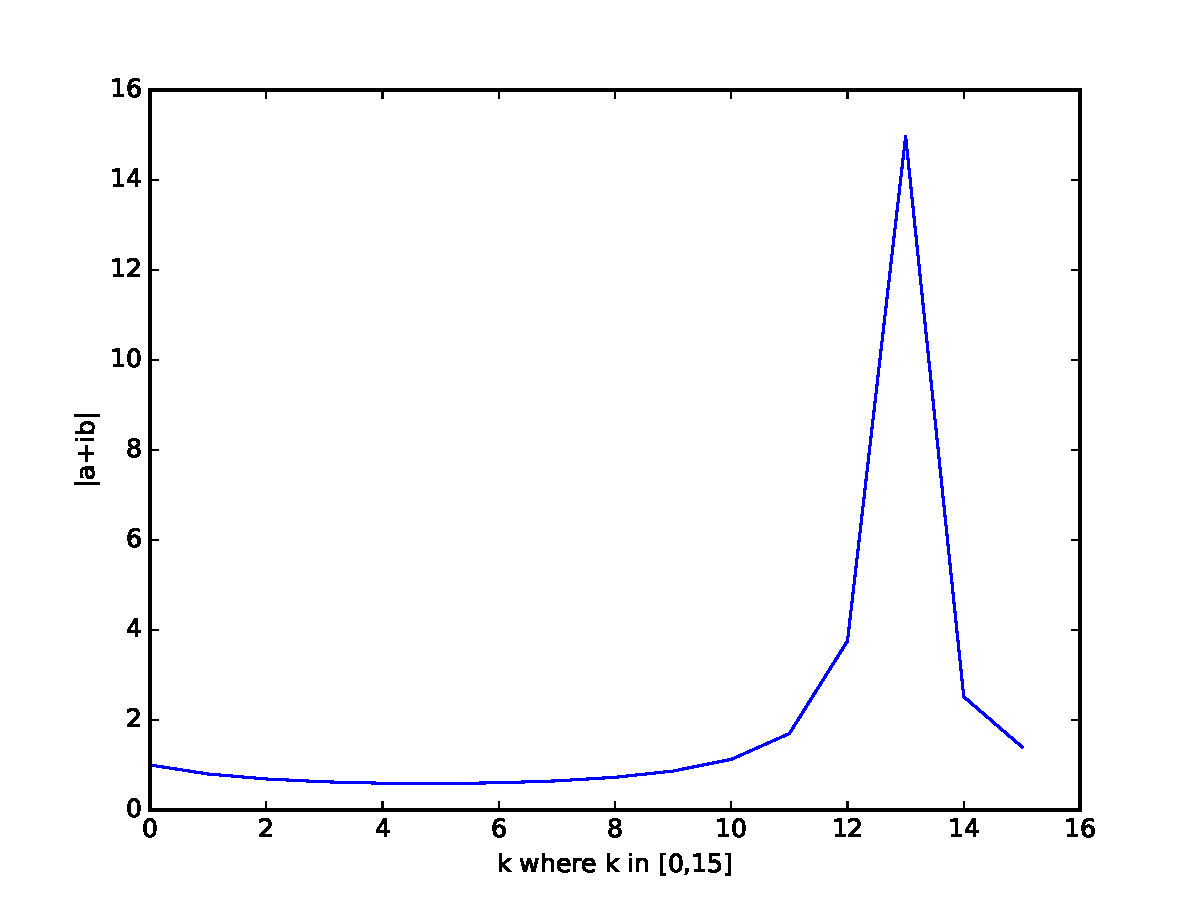
\includegraphics[scale=.5]{fig2.pdf}
 % abs.pdf: 0x0 px, 300dpi, 0.00x0.00 cm, bb=
\end{center}\begin{center}
 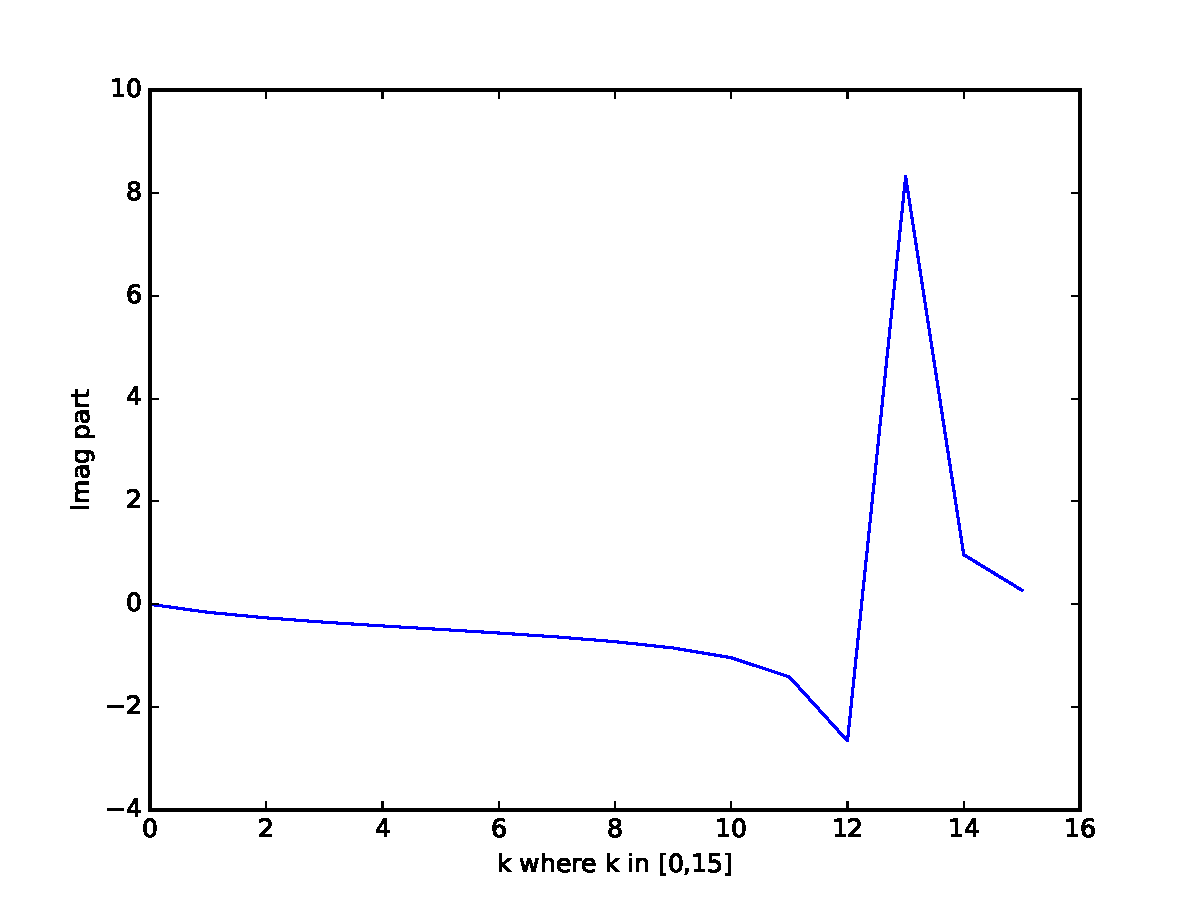
\includegraphics[scale=.5]{fig4.pdf}
 % imag.pdf: 0x0 px, 300dpi, 0.00x0.00 cm, bb=
\end{center}
\begin{center}
 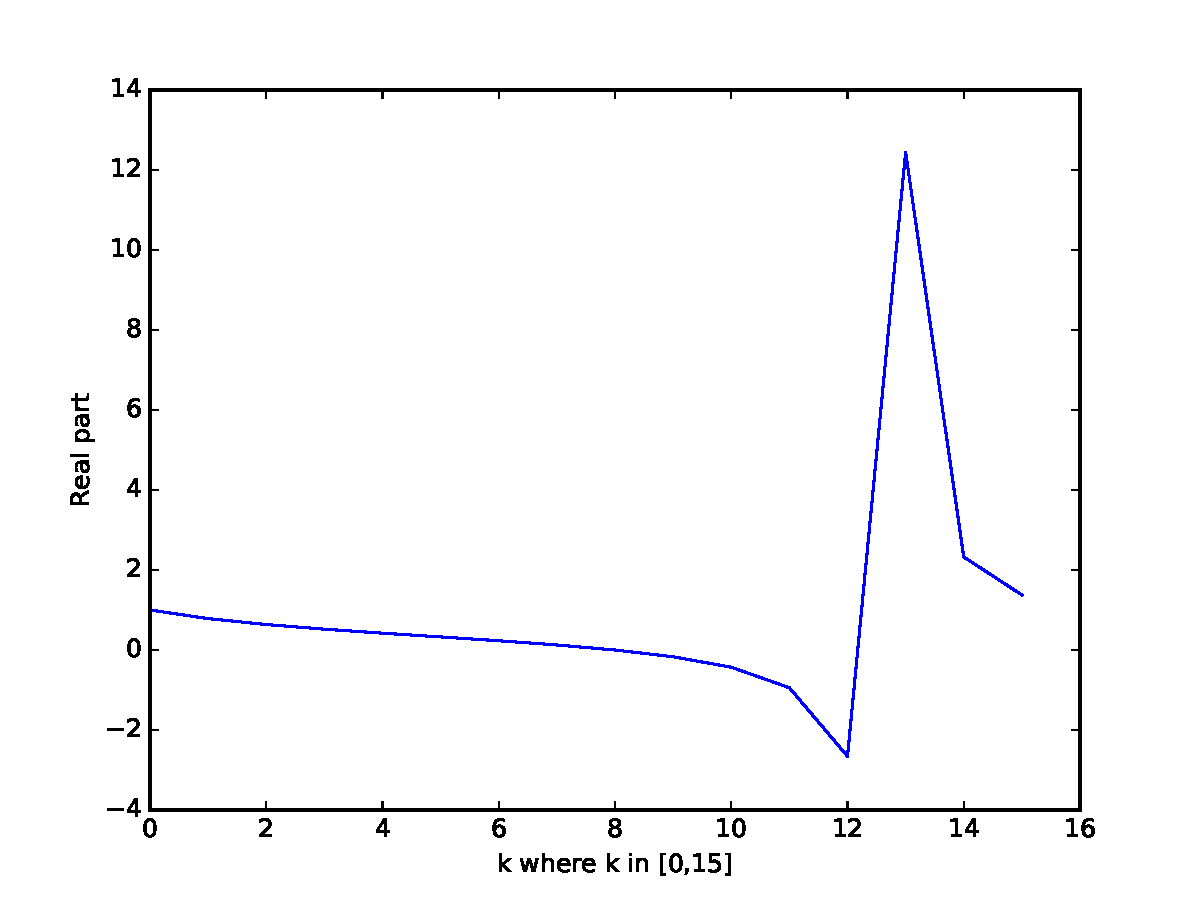
\includegraphics[scale=.5]{fig3.pdf}
 % real.pdf: 0x0 px, 300dpi, 0.00x0.00 cm, bb=
\end{center}
\begin{center}
 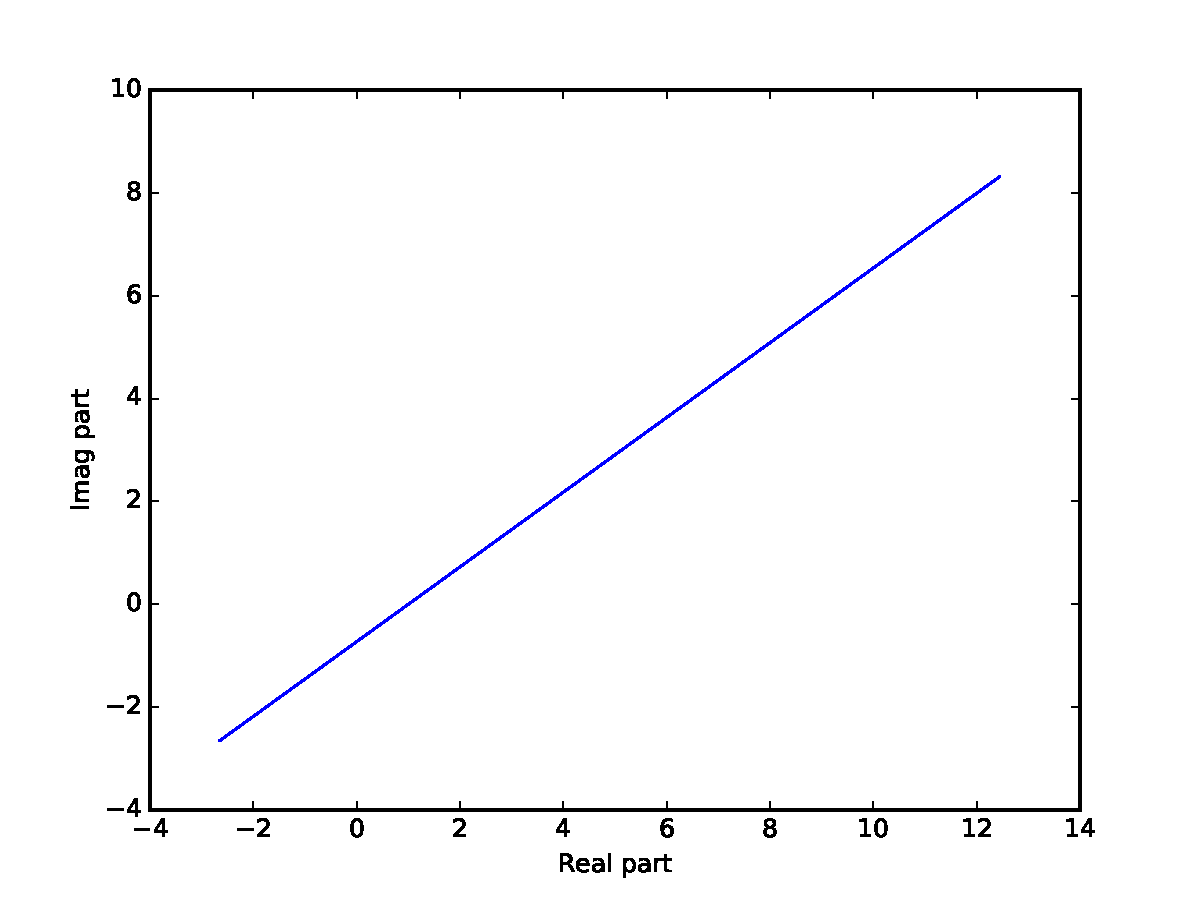
\includegraphics[scale=.5]{fig1.pdf}
 % realvIm.pdf: 0x0 px, 300dpi, 0.00x0.00 cm, bb=
\end{center}
Observation: Graph of real and imaginary part is a straight line, the imaginary and real graph has a peak around t = 1/f, f = .2

\end{document}
